\documentclass[runningheads,a4paper]{llncs}

\usepackage[english, USenglish, american]{babel}
\usepackage{ucs}
\usepackage{forest} % for diagrams
\usepackage{tikz-qtree} % for digramas
\usepackage{framed}
\usepackage[utf8x]{inputenc} 							% Encoding (allows accents)
\usepackage[printonlyused,nolist]{acronym}	% Acronyms (print only used)
\usepackage{cite}% Allow multiple citations, etc.
\usepackage{indentfirst} 								% Allow indent on first paragraph
% \usepackage[pdftex]{graphicx}
\usepackage{graphicx} 									% Pictures
\usepackage[cmex10]{amsmath}
\usepackage{amssymb}
\usepackage{mathtools}									% Maths
\usepackage{algorithmic}
\usepackage{algorithm}
\usepackage{array}
\usepackage{mdwmath}
\usepackage{mdwtab}
\usepackage{eqparbox}
\usepackage{longtable}
\usepackage{lscape}
\usepackage{rotating}
\usepackage[raggedright]{sidecap} % for side captions
\usepackage{multirow}
\usepackage{hyphenat}
\usepackage{alltt}
\usepackage{booktabs}
\usepackage[tight,footnotesize]{subfigure}
\usepackage[hyphens]{url}
\usepackage{pdflscape}									% Allow horizontal pages (in the pdf too)
\usepackage[breaklinks=true]{hyperref}
\usepackage{color}
\usepackage[left]{lineno}
\usepackage[textwidth=2.8cm,disable]{todonotes}
\setcounter{tocdepth}{3}
\hyphenation{op-tical net-works semi-conduc-tor}
\setlength{\parindent}{0.5cm}
\setcounter{secnumdepth}{3}
\selectlanguage{USenglish}
\newcommand{\keywords}[1]{\par\addvspace\baselineskip
\noindent\keywordname\enspace\ignorespaces#1}
\usepackage{caption} 
\captionsetup[table]{skip=5pt}
\usepackage{listings} 									% Source code blocks
\usepackage[toc,page]{appendix}							% Appendix
\usepackage{qtree}
\usepackage{newfloat}
\usepackage{bm}
\usepackage{verbatim}

\newlength{\wideitemsep}
\setlength{\wideitemsep}{\itemsep}
\addtolength{\wideitemsep}{+10pt}

\newcommand{\tallitem}{\setlength{\itemsep}{\wideitemsep}\item}
\renewcommand{\arraystretch}{1.2} % increase space in tables
\setlength{\tabcolsep}{.25em} % increase horizontal space in tables

%\makeatletter
%\renewcommand\subsubsection{\@startsection{subsubsection}{3}{\z@}%
%	{-18\p@ \@plus -4\p@ \@minus -4\p@}%
%	{4\p@ \@plus 2\p@ \@minus 2\p@}%
%	{\normalfont\normalsize\bfseries\boldmath
%		\rightskip=\z@ \@plus 8em\pretolerance=10000 }}
%\renewcommand\paragraph{\@startsection{paragraph}{4}{\z@}%
%	{-12\p@ \@plus -4\p@ \@minus -4\p@}%
%	{2\p@ \@plus 1\p@ \@minus 1\p@}%
%	{\normalfont\normalsize\itshape
%		\rightskip=\z@ \@plus 8em\pretolerance=10000 }}
%\makeatother


\begin{document}

%%%%%%%%%%%%%%%%%%%%%%%%%%%%%%%%%%%%%%%%%%%%%%%%%
% For REVIEW
% \linenumbers
%%%%%%%%%%%%%%%%%%%%%%%%%%%%%%%%%%%%%%%%%%%%%%%%%

%%%%%%%%%%%%%%%%%%%%%%%%%%%%%%%%%%%%%%%%%%%%%%%%%
% fix TOC on llncs
\makeatletter
\renewcommand*\l@author[2]{}
\renewcommand*\l@title[2]{}
\makeatletter
%%%%%%%%%%%%%%%%%%%%%%%%%%%%%%%%%%%%%%%%%%%%%%%%%

\mainmatter

\urldef{\mailsa}\path|nuno.xu@tecnico.ulisboa.pt|

\title{Trust Model for Human Agent Interaction}
\authorrunning{Trust Model for Human Agent Interaction}
% (feature abused for this document to repeat the title also on left hand pages)

\author{Nuno Xu\\
	\mailsa}

\institute{
	\textbf{Supervisors}: Rui Prada and Ana Paiva\\
	Técnico Lisboa (Taguspark)\\
	Universidade de Lisboa\\
	Av. Prof. Dr. Aníbal Cavaco Silva\\ Porto Salvo, Portugal\\
	\url{http://tecnico.ulisboa.pt/en/}\\
}

%\begin{comment}
%\pagenumbering{gobble}
\maketitle
%\begin{abstract}
Trust is an essential ingredient for cooperation and collaboration, so if we want to further develop autonomous collaborative agents we must address the issue of trust in such relationships. For that reason, computational trust has seen a great spike of interest in recent years, however the literature has been only focused in issues like design, animation and modelling. We aim to address the uncharted matter of actively improve trust by proposing a module capable of suggesting actions to the agent. The suggestions be must based on our beliefs of the user towards the agent, therefore we will also need a trust model of the user. So in this report we explore the state of the art in trust modelling and decision making, while defining the major concepts used in the literature. Afterwards we discuss our solution and its basis on the Repage architecture. Finally project evaluation is planned out and scheduled.

\keywords{Artificial Intelligence, Trust, \acl{HAI}, Decision Making}
\end{abstract}

%%%%%%%%%%%%%%%%%%%%%%%%%%%%%%%%%%%%%%%%%%%%%%%%%
% Table of content
%\newpage
%\tableofcontents
%\newpage
%%%%%%%%%%%%%%%%%%%%%%%%%%%%%%%%%%%%%%%%%%%%%%%%%
%\end{comment}
%\pagenumbering{arabic}
\section{Introduction}
\label{sec:Introduction}

% TODO - Insert motivation on the topic:
% - while a lot of reasearch has been done in modeling trust and in automation, little  research trust in HAI has been found
% - trust is an important component of the social fabric, and essential if we want to have collaboration
% - mention that people tend to "anthropomorphize" computers, applying social rules in computer interactions so trust becomes an interesting concern as shown in \cite{Reeves1998a} and \cite{Fogg1997}
% - First paragraph - Say that trust is a fundamental part of social interaction, and as agents try to simulate this,and by this reason there's been quite some focues in computational trust during recent years, (cite reviews). Give applications of the trust models (specially on e-commerce)
% - Second paragraph - Briefly say what has been done (not too much, leave for related work) and comment on what is lacking.
% - Third paragraph - Introduce your solution, and why it's going to improve the field. Relate to the comments mentioned previously
% - Fourth paragraph - Finally give the structure of the paper (and it's scope? check if hay is needed...)
Trust has been described in Psychology as being one of the most important components of interpersonal relationships \cite{Simpson2007}. It is undeniable the need of Trust to promote cooperation and collaboration between two parties, either in deciding who should one collaborate with, or even on what exactly do we trust the other party with. 


As \ac{AI} Research gravitates towards the development of Intelligent Agent Systems \cite{Russell2009a}, where a focal concern is the performance of collaborative tasks\cite{Grosz1996, Allen2002, Allen2007}, as well as addressing the problems of interaction between humans and agents\cite{Bradshaw2011}, one would consider that Trust should be one of the main focuses of \ac{HAI}. Since the start of automated machinery, one of the main issues was how to properly manage trust on machines, in order to avoid over or under reliance\cite{Lee2004}. Reeves and Nass have shown that people apply social rules to \ac{HCI}, and this can logically be extended to the sub-field of \ac{HAI}\cite{Reeves1998a}. So as agents evolve to better perform collaborative tasks with humans autonomously, which demands at least some amount of social interaction, the active agent must seek out to improve the trust relationship it has with the user \cite{Lashkari1994}. And while the amount of literature has been increasing, we found it surprising that not enough work has been done in \ac{HAI} focusing on Trust, other than on design issues\cite{Bickmore2005} and the sub-field of \ac{HRI}\cite{Goodrich2007, VandenBrule2014}, specially when so much has been done regarding Trust in Automation \cite{Lee1992, Jones1997, Lee2004}. This reveals that while the area has so much potential, the level of understanding is still very shallow, only deeply focused in specific areas.

\ac{MAS} Trust and Reputation modelling is one of the areas that has been having a great increase of interest lately, specially ever since the advent of \ac{P2P} e-commerce in platforms like \textit{E-bay}\cite{eBay2002}, where tools and solutions to ensure trust were needed for a new reality of a mass amount of anonymous entities constantly entering and exiting the environment and performing trading transactions through an open space. However almost all research focuses purely on the creation and maintenance of the internal trust model structure of the agent, normally with just the purpose of ranking other agents, through the use of statistical and game theoretical based methods. This makes it difficult to create a model that is easy to understand, analyse and, most importantly, describe its evaluative reasoning in a human understandable manner. The introduction of cognitive models by Castelfranchi and Falcone \cite{Castelfranchi1998} tries to solve that problem, mapping the trust model to the agent's mental state, composed by beliefs and goals, very akin to existing cognitive agent architectures like BDI\cite{Rao1995}. Then some systems, like Repage\cite{Sabater2006}, created implementations of this new paradigm of trust modelling; until then most of the models were purely theoretical. Nevertheless, there is a gap in this area of research that we wish to address with our work, and that is the lack of an implementation for an action suggester based on the agent's trust model to improve the strength of our beliefs in the model and to improve trust in our agent. While one could argue that this is the responsibility of the decision making or planner component of the agent, we believe that a dedicated module will ease the complexity of decision by making it more modular, and also allowing for a greater degree of integration with the trust model of the agent. To our knowledge, no attempts have been done towards this goal, so we propose to develop two agent modules: firstly, one capable of creating a cognitive model representing the mental state of the user's trust in the agent, using Repage's architecture, and secondly, another to suggest what actions should be used to improve trust on the agent. We will ascertain this project's objectives by integrating the modules in an agent implementation (currently finishing development in our research group, \acs{GAIPS}\footnote{\ac{GAIPS}: \url{http://gaips.inesc-id.pt/}}) that is capable of acting as one of the players in the \textit{Split or Steal} scenario, introduced in the British game show \textit{Golden Balls}\cite{Wikipedia.Golden.Balls}, the scenario is further described in Section \ref{subsec:Evaluation:Split or Steal}. 

We hope that this project will make agent decision making more interesting, provide some insight on how actions affect trust and budge the field a bit in this unexplored direction.


\subsection{Goals}
\label{subsec:Goals}
% Clearly state what must be done to consider this thesis a success (may prove difficult as it's too abstract) maybe focus on objective marks on trust improvement of the subject.
% Need to go fetch what is the trust measurement questionaires.

% we aim to create a generic agent model that combines the already extensive reasearch in trust modeling in MAS systems with a decision making module with strategies to improve trust in the agent.
% we want to focus on human to agent interaction. so improve and model human trust.
% find out which parameters and features can be explicitly chosen to human modeling.
In sum, this project's purpose will be to:
\begin{itemize}
	\item Create a cognitive trust model capable of representing human trust towards the agent using the Repage architecture;
	\item Develop an action suggestion module that aims to provide actions that improve trust in the agent (or a least the beliefs on this trust);
	\item Calibrate the modules through user testing in the \textit{Split or Steal} scenario.
\end{itemize}


In the remainder of the document we will present a brief summary of the main concepts used in this project in Section \ref{sec:Background}. Then in Section \ref{sec:Related Work} we will discuss some of the work done in modelling trust for \acp{MAS} and measuring trust in \ac{HRI} applications. In Section \ref{sec:Solution} a description of our solution architecture will be presented, followed by our plans and schedules in Section \ref{sec:Planning}. Finally in Section \ref{sec:Evaluation} we will describe how we will evaluate the project.



\section{1st Model}
\label{sec:Model}

In an effort to create a working trust model iteratively, we will start by simplifying the model described by Castelfranchi and Falcone \cite{Castelfranchi1998}, by removing the effects of outside influence in Trust representation. We also do not take into account long term considerations of the trustor's goal, reducing contextual scope to just the task being performed by the trustor. So Trust is represented by a 3-tuple:

\begin{itemize}
	\item The trustor (\textbf{X});
	\item The trustee (\textbf{Y});
	\item A task ($\bm{\tau}$) defined by the pair $(\alpha, \rho)$, where \bm{$\alpha$} is the action entrusted to the trustee, that possibly produces an outcome \bm{$\rho$}, contained in the goal of X.
\end{itemize}
\begin{equation}
TRUST(X\ Y\ \tau)
\label{eq:TrustRelation}
\end{equation}

We seek to represent the trustee as a collection of features from which an overall evaluation may be retrieved. These features provide a representation of the trustee's abilities in various fields, as well as concerns related to willingness, such as task preference, for example, a trustee $Y$'s feature set $ F_y $ can be as seen in \ref{eq:FeaturesExample}.

\begin{equation}
F_y=\left\{cooking, writing, preference\ to\ cook\right\}
\label{eq:FeaturesExample}
\end{equation}

This makes visualization of a certain trustee's trust reasoning, as we can observe all the factors that contribute towards an evaluation. The specificity of the concrete features is purposefully left generic in order make the model fit in different scenarios. This makes the model dependent on an ontology specific for the scenario, but we think this concern is unavoidable if we want to have understandable models, as the alternative solution is to use machine learning to perform clustering, which provi. These features must be able to provide 2 values:

\begin{itemize}
	\item trust - a value for how much trust we have in this trustee's specific feature;
	\item certainty - the degree of how much we believe this trust assumption to be true, as factors like how many times, or how long ago, did we last affirm this belief may affect the believability of our assumptions.
\end{itemize}
\begin{figure}[hbt]
	\centering
	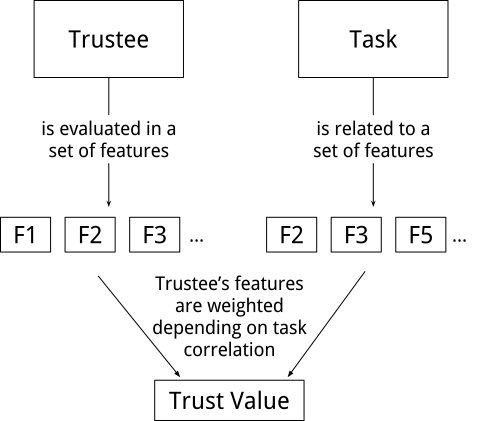
\includegraphics[height=200px]{figures/Trust_Model_Diagram.png}
	\caption{Trustee Features Representation}
	\label{fig:trustee}
\end{figure}

Trust and certainty are calculated through a collection of belief sources, which in the first version will be a history of direct contacts. The environment must be able to provide some way to access these contacts, either by a callback function or through open access to an action history. If the environment does not provide such features, a perception module, capable of checking action results, will be required.

The task is composed by a set of related features with a given weight. This represents the features most closely related to the task at hand, and their importance to he completion of the task.

\subsection{Implementation}

Implementation wise, the model will be first implemented by using a simple class structure, as seen in figure \ref{fig:classDiagram}. In this diagram, the main actor is the Agent, which contains a list of Trustees with features that the Agent has been able to perceive from received sources. For now the sources must be given by the simulation environment, but an interpreter should be implemented to sort out and transform the perceptions received by the environment into sources for belief features.
A simple simulation example can be performed as following:
\begin{enumerate}
	\item Instantiate Agent A(nna) and Agent B(ob);
	\item Instantiate Trustee B and assign as A's trustee;
	\item Insert Direct Contact Source with Feature ID "Cooking"; this should create a new Trust Feature in Trustee B;
	\item Calculate Trust with task "Cook";
\end{enumerate}

\begin{figure}[hbt]
	\centering
	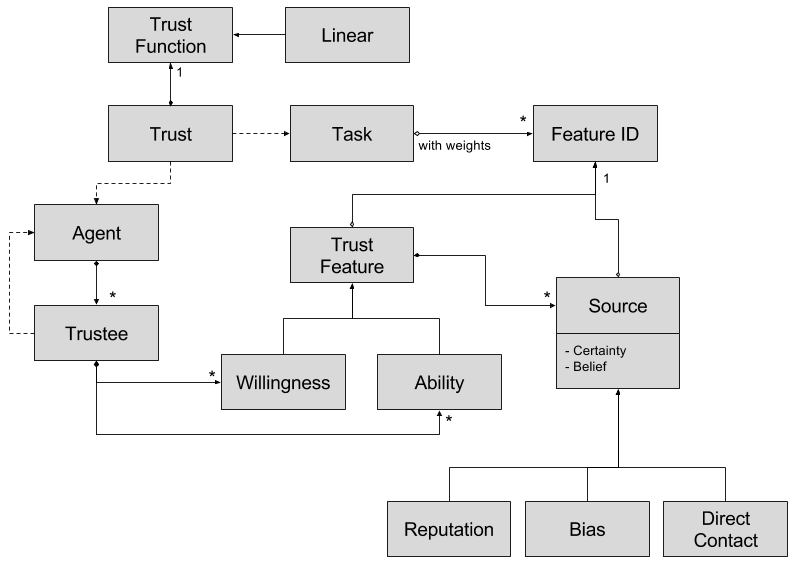
\includegraphics[height=250px]{figures/Class_Diagram.png}
	\caption{Class Diagram}
	\label{fig:classDiagram}
\end{figure}

\section{Example Case}




\section{Conclusion}
\label{sec:Conclusion}
We started by introducing our thoughts about the lack of research done in the area of trust in \ac{HRI}, especially regarding trust improvement, and how we want to address that issue by tackling one of the gaps exposed in the research: action suggestion to improve trust and their beliefs. So we summed up our main goal as to develop an action suggestion module capable of giving out actions that will improve trust in the agent. Then we went on to establish some background concepts specific to the domain, like the definitions of trust and what we think it is more appropriate for our work, as there is no literary consensus on which one is the best. Afterwards we delved into the related work we found about trust models in \acp{MAS}, 


%%%%%%%%%%%%%%%%%%%%%%%%%%%%%%%%%%%%%%%%%%%%%%%%%
% References
\newpage
\bibliographystyle{splncs}
\bibliography{bib/IEEEabrv,bib/library}
%%%%%%%%%%%%%%%%%%%%%%%%%%%%%%%%%%%%%%%%%%%%%%%%%

%\listoftodos

% This is the ACRONYMS Definition
\begin{acronym}[TDMA]
	\acro{GAIPS}{Intelligent Agents and Synthetic Characters Group}
	\acro{ML}{Machine Learning}
	\acro{SVM}{Suport Vector Machine}
	\acro{HRI}{Human Robot Interaction}	
	\acro{HAI}{Human Agent Interaction}
	\acro{HCI}{Human Computer Interaction}
	\acro{CTM}{Cognitive Trust Model}
	\acro{MAS}{Multi-Agent System}
	\acro{NLP}{Natural Language Processing}	
	\acro{AI}{Artificial Intelligence}	
	\acro{DoC}{Degree of Credibility}
	\acro{DoT}{Degree of Trust}
	\acro{SBH}{Social Brain Hypothesis}
	
	
	
	%%%%%%%%%%%%%%%
	\acro{AAC}{Advanced Audio Coding}
	\acro{ADTS}{Audio Data Transport Stream}
	\acro{AS}{Application Server}
	\acro{AV}{Audio-Visual}
	\acro{AVC}{Advanced Video Coding}
	\acro{BMFF}{base media file format}
	\acro{CASHED}{Cloud-Assisted Adaptive and Scalable Video Streaming for Heterogenous End-User Devices}
	\acro{CC}{Cloud Computing}
	\acro{CDN}{Content Distribution Network}
	\acro{CPU}{Central Processing Unit}
	\acro{DASH}{Dynamic Adaptive Streaming over HTTP}
	\acro{DVD}{Digital Versatile Disk}	
	\acro{ES}{Elementary Stream}
	\acro{ESM}{End System Multicast}
	\acro{ftyp}{File Type}
	\acro{FLV}{Flash Video}
	\acro{GPRS}{General Packet Radio Service}
	\acro{GSM}{Global System for Mobile Communications}
	\acro{H.264/AVC}{Advanced Video Coding}
	\acro{H.264/SVC}{Scalable Video Coding}
	\acro{HD}{High Definition}
	\acro{HDTV}{High Definition Television}
	\acro{HLS}{HTTP Live Streaming}
	\acro{HTTP}{Hypertext Transfer Protocol}
	\acro{IaaS}{Infrastructure as a Service}
	\acro{IETF}{Internet Engineering Task Force}
	\acro{IGMP}{Internet Group Management Protocol}
	\acro{IIS}{Internet Information Services}
	\acro{IMS}{IP Multimedia Subsystem}
	\acro{IP}{Internet Protocol}
	\acro{IPTV}{IP Television}
	\acro{ISP}{Internet Service Provider}
	\acro{IT}{Information Technology}
	\acro{JSVM}{Joint Scalable Video Model}
	\acro{LAN}{Local Area Network}
	\acro{LTE}{Long Term Evolution}
	\acro{MDC}{Multiple Description Coding}
	\acro{MIB}{Management Information Bases}
	\acro{MIME}{Multipurpose Internet Mail Extension}
	\acro{MOS}{Mean Opinion Score}
	\acro{MPD}{Media Presentation Description}
	\acro{MPEG}{Moving Picture Expert Group}
	\acro{MVC}{Multi-View Coding}
	\acro{NAL}{Network Abstraction Layer}
	\acro{NAT}{Network Address Translation}	
%	\acro{NAL}{Network Access Layer}
	\acro{OS}{Operating System}
	\acro{OSMF}{Open Source Media Framework}
	\acro{P2P}{Peer-to-Peer}
	\acro{P2P}{Peer-To-Peer}
	\acro{PPSP}{Peer-to-Peer Streaming Protocol}
	\acro{PaaS}{Platform as a Service}
	\acro{PES}{Packetized Elementary Streams}
	\acro{QoE}{Quality Of Experience}
	\acro{QoS}{Quality Of Service}
	\acro{QP}{Quantization Parameter}
	\acro{RMON}{Remote Monitoring}
	\acro{RTCP}{RTP Control Protocol}
	\acro{RTMP}{Real Time Messaging Protocol}
	\acro{RTP}{Real-time Transport Protocol}
	\acro{RTSP}{Real Time Streaming Protocol}
	\acro{SaaS}{Software as a Service}
	\acro{SD}{Standard Definition}
	\acro{SEI}{Supplemental Enhancement Information}
	\acro{SIP}{Selective Inter-layer Prediction}
	\acro{SMS}{Short Message Service}
	\acro{SNMP}{Simple Network Monitoring Protocol}
	\acro{SNR}{Signal-to-Noise Ratio}
	\acro{SVC}{Scalable Video Coding}
	\acro{TCP}{Transport Control Protocol}
	\acro{TS}{Transport Stream}
	\acro{TTL}{Time-to-Live}
	\acro{UDP}{User Datagram Protocol}
	\acro{UI}{User Interface}
	\acro{UMTS}{Universal Mobile Telecommunication System}
	\acro{URL}{Uniform Resource Locator}
	\acro{VCEG}{Video Content Expert Group}
	\acro{VCL}{Video Coding Layer}
	\acro{VoD}{Video On Demand}
	\acro{WAN}{Wide Area Nework}
	\acro{WLAN}{Wireless Local Area Network}
	\acro{WMA}{Windows Media Audio}
	\acro{WWAN}{Wireless Wide Area Network}		
	\acro{XML}{Extensible Markup Language}
\end{acronym}

%%%%%%%%%%%%%%%%%%%%%%%%%%%%%%%%%%%%%%%%%%%%%%%%%
% Appendices
\newpage
\appendix
\section*{Appendices}
\section{Variants of Single-subject designs}

\newpage
\begin{landscape}
	\section{Landscape Appendice}
	\label{app:Educational}	
	landscape page
\end{landscape}

\newpage
\section{The Perception and Measurement of Human-Robot Trust: Items Table}

\begin{longtable}{l|l}
	\multicolumn{1}{c|}{\textbf{Items}} & \textbf{Perceived as relevant} \\ \hline
	\endhead
	Act consistently & \\ \hline
	Protect people & \\ \hline
	Act as part of the team & \\ \hline
	Function successfully & \\ \hline
	Malfunction & \\ \hline
	Clearly communicate & \\ \hline
	Require frequent maintenance & \\ \hline
	Openly communicate & \\ \hline
	Have errors & \\ \hline
	Perform a task better than a novice human user & \\ \hline
	Know the difference between friend and foe & \\ \hline
	Provide Feedback & \\ \hline
	Possess adequate decision- making capability & \\ \hline
	Warn people of potential risks in the environment & \\ \hline
	Meet the needs of the mission & \\ \hline
	Provide appropriate information & \\ \hline
	Communicate with people & \\ \hline
	Work best with a team & \\ \hline
	Keep classified information secure & \\ \hline
	Perform exactly as instructed & \\ \hline
	Make sensible decisions & \\ \hline
	Work in close proximity with people & \\ \hline
	Tell the truth & \\ \hline
	Perform many functions at one time & \\ \hline
	Follow directions & \\ \hline
	Considered part of the team & \\ \hline
	Responsible & \\ \hline
	Supportive & \\ \hline
	Incompetent & \\ \hline
	Dependable & \\ \hline
	Friendly & \\ \hline
	Reliable & \\ \hline
	Pleasant & \\ \hline
	Unresponsive & \\ \hline
	Autonomous & \\ \hline
	Predictable & \\ \hline
	Conscious & \\ \hline
	Lifelike & \\ \hline
	A good teammate & \\ \hline
	Led astray by unexpected changes in the environment & \\
	\caption{The Perception and Measurement of Human-Robot Trust: Items Table}
	\label{app:measurement.items.table}	
\end{longtable}

%%%%%%%%%%%%%%%%%%%%%%%%%%%%%%%%%%%%%%%%%%%%%%%%%

\end{document}